\chapter{Gesamtkonzept Softwareplattform}

In diesem Kapitel wird anhand der Anforderungen aus dem Forschungsansatz eine Gesamtarchitektur des Softwareplattforms vorgestellt, sowie die Softwarearchitektur der beiden Softwarekomponenten \enquote{Runtime Node} und \enquote{Runtime Master}. 

\section{Verteiltes Rechenplattform aus autonomen Fahrzeugsteuergeräten}

Die Rechenleistung von autonomen Fahrzeugen kann in verschiedenen Nutzungskonzepten verwendet werden. Im Kapitel \autoref{Hardwareumgebung in Fahrzeugen} wurde die Hardware vorgestellt, die typischerweise in autonomen Fahrzeugsteuergeräten zu finden ist. Es wird deutlich, dass diese Steuergeräte über Hardwaremodule verfügen, die die Rechenleistung für spezifische Rechenoperationen erhöhen. Grafikprozessoren beinhalten viele Rechenkerne, die parallel auf gro0en Datenmengen opreationen ausführen können. In den meisten Architekturen können die GPU-Cores nur in Gruppen verwendet werden, wobei jede Gruppe die gleiche Rechenoperation ausführen muss. Kerne für Neuronale Netzwerk Berechnungen implementieren Matrix Operationen in Hardware, so dass diese in erheblich weniger Rechenzyklen als bei sequentieller Berechnung durchgeführt werden können. Folglich können nur solche Rechenaufgaben sinnvoll auf diese Steuergeräte ausgelagert werden, die sich in viele parallele Berechnungen aufteilen lassen. Typische Beispiele für solche Berechnungen sind:

\begin{itemize}
    \item Mathematik: Vektor und Matrixoperationen
    \item Bildbearbeitung: FFT oder Faltungsoperationen
    \item Simulation: Moleküldynamik, Finite-Elemente Analyze, Fluiddynamik
    \item Finanzsegment: Monte Carlo Simulation, Optionspreisgestaltung, Portfolio Optimierung
    \item Kryptographie und Sicherheit: Hashing Algorithmen, Passwortknacken, Blockchain und Kryptowährung Mining
    \item Datenanalyse in Naturwissenschaften: Genomische und bioinformatische Berechnungen, Big Data Verarbeitung
    \item Optimerung: Genetische Algorithmen Berechnungen
    \item Quantum Computing: Simulation von Quantumsystemen
\end{itemize}

Die Neuronale Netzwerk Beschleuniger können zudem für das Trainieren von neuronalen Netzwerken effizient verwendet werden. 

Trotz der Einschränkung in der Art der Rechenaufgaben, die auf der Hardware effizient berechnet werden können, ergibt sich eine Vielzahl möglicher Anwendungsszenarien. Die ungenutzte Rechenleistung kann also von verschiedenen Kunden sinnvoll verwendet werden. Folgende Ansätze für die Bereitstellung der Ressourcen an Kunden wären Denkbar:

\begin{itemize}
    \item Nutzung ausschließlich durch den Hersteller: Diese Methode ist die transparenteste und sicherste Methode für den Fahrzeughersteller. Nur der Hersteller selber Applikationen auf die Fahrzeuge ausrollen und die ungenutzte Rechenleistung nutzen
    \item Nutzung durch Hersteller und ausgewählte Kunden: Der Hersteller stellt die Rechenleistung auch an ausgewählte Kunden zur Verfügung, hierbei vertraut der Hersteller den Kunden, dass sie keine illegale Aktivitäten ausüben und nicht aktiv Versuchen Schutzmechanismen des Systems umzugehen.
    \item Nutzung durch frei verfügbaren Marktplatz: Beliebige Kunden können auf dem Marktplatz Rechenleistung einkaufen. In diesem Konzept muss sichergestellt werden dass Kunden keine illegale Aktivitäten ausüben und dass sie die Sicherheitsmechanismen des Plattforms nicht versuchen zu umgehen.
\end{itemize}

Für die ersten Versionen einer solchen Plattform kommen realistischerweise nur die ersten beiden Möglichkeiten in Frage. Eine freie Nutzung erfordert sehr hohe Sicherheitsstandards für die Plattform, die mit erheblichem Entwicklungs- und Erfahrungsaufwand verbunden sind. 

Die Nutzung freier Rechenressourcen erhöht den Stromverbrauch des Fahrzeugs. Daher müssen Anreize für die Nutzer geschaffen werden, die Rechenleistung des Fahrzeugs freizugeben. Hier können ähnliche Konzepte wie in der Informatik verwendet werden. Es gibt verschiedene Plattformen, auf denen PC-Nutzer ihre Rechenleistung zur Verfügung stellen können. 

Plattformen, die auf freiwilliger Teilnahme und Bereitstellung von Rechenressourcen beruhen, haben sich als erfolgreich erwiesen. Voraussetzung ist, dass die Rechenleistung nur für Zwecke eingesetzt wird, die von der Gesellschaft als gemeinnützig und sinnvoll erachtet werden. Ein verbreitetes Beispiel ist das Projekt \gls{BOINC}. In diesem Projekt können Nutzer ihre ungenutzte Rechenleistung für verschiedene naturwissenschaftliche Projekte zur Verfügung stellen. \gls{BOINC} stellt die Rechenleistung für verschiedene Anwendungen in Bereichen wie Medizintechnik, Biologie, Mathematik, Linguistik, Klimaforschung, Umweltwissenschaften, Astrophysik zur Verfügung. Die teilnehmenden Nutzer erhalten Punkte für die im Projekt erbrachte Rechenleistung. Diese Punkte können jedoch nicht eingelöst werden und dienen lediglich der Nachvollziehbarkeit und Vergleichbarkeit der erbrachten Rechenleistung unter den Nutzern. Ein ähnliches Konzept könnte daher auch für die Nutzung der freien Rechenleistung von Fahrzeugen erfolgreich sein, sofern die Rechenleistung für gemeinnützige Zwecke genutzt wird.

Wenn eine kommerzielle Nutzung der Rechenleistung vorgesehen ist, müssen die Nutzer, die Rechenleistung zur Verfügung stellen, entlohnt werden. Viele Plattformen im IT-Bereich setzen dabei auf die Bezahlung mit Kryptowährungen. Dies hat den Vorteil, dass die Zahlungsbedingungen direkt im Blockchain-Vertrag festgehalten werden können, sodass kein Vertrauen in die Einhaltung der Bedingungen durch den Plattformbetreiber erforderlich ist. Exemplarisch kann in diesem Kontext das Golem-Projekt betrachtet werden. 

Das Konzept sieht die Implementierung eines Markplatzes vor, wo Benutzer Rechenleistung einkaufen und verkaufen können. Die Erstellung der Rechenaufgaben kann auf zwei verschiedene Arten erfolgen. Entweder werden bereits kompatible Funktionscodes in Form von Vorlagen genutzt, oder die Funktionscodes werden vom Benutzer implementiert. Die Aufgabenverwaltung registriert die neue Aufgabe, welche durch einen Benutzer angestoßen wurde. Der Benutzer, der die Rechenleistung der Plattform in Anspruch nehmen möchte, erstellt ein Angebot, in dem er die Höhe der Vergütung angibt. Diese Angebote werden auf dem Netzwerk an allen Benutzer übertragen, die Rechenleistung zur Verfügung stellen. Zusätzlich kann das Angebot Einschränkungen bezüglich der Hardware oder geographische Lage beinhalten.

Die Bereitstellung von Rechenleistung erfolgt durch die lokalen Ausführungen eines Transaktionssystem-Moduls durch die jeweiligen Benutzer. Dieser Modul sammelt alle verfügbaren Aufgabenangebote im Netzwerk und wählt das beste Angebot aus. Des Weiteren verfügt auch derjenige, der ein Angebot erstellt, über eine Reputation auf der Plattform. Angebote von Benutzern, deren Reputation als zu gering erachtet wird, werden abgelehnt. Sofern alle Anforderungen des Angebots durch den Rechenleistung-Bereitsteller erfüllt sind, wird das Angebot angenommen. 

Die Rechenaufgabe, inklusive benötigte Ressourcen wird auf den PC vom Rechenleistung-Bereitsteller heruntergeladen. Der PC berechnet im Anschluss die entsprechende Aufgabe. Der Rechenleistung-Bereitsteller kann die geladenen Anwendungen in verschiedenen Umgebungen ausführen. Es kann eine Virtualisierungsmethode wie Container oder virtuelle Maschine verwendet werden, um die Anwendungen vom Hostsystem zu isolieren, oder es kann direkt auf dem Hostsystem ausgeführt werden, wenn die Anwendung als vertrauenswürdig eingestuft wird. 

Nach der Berechnung der Aufgabe werden die Ergebnisse und Protokolle an den Auftraggeber zurückgeschickt. Die Aufgabenverwaltung validiert die Ergebnisse, indem entweder Teile der Aufgabe von anderen Teilnehmern redundant berechnet werden oder Teile lokal berechnet und überprüft werden. Sind die Ergebnisse erfolgreich validiert, wird der Benutzer, der die Rechenleistung erbracht hat, entsprechend dem Angebot bezahlt. Falls die Ergebnisse nicht korrekt sind, wird die Reputation des Rechenleistung-Bereitstellers verringert. 

Ein Konzept wie es im Golem-Projekt umgesetzt wurde, eignet sich auch für die Bereitstellung von Fahrzeugrechenressourcen im kommerziellen Einsatz. Dieses Konzept kann vereinfacht werden, wenn die Plattform vom Hersteller betrieben wird. Der Hersteller kann eine zentrale Zahlungsinstanz betreiben, so dass keine Kryptowährung als Zahlungsmittel verwendet werden muss. In diesem Fall wird der Hersteller als vertrauenswürdiger Betreiber angesehen, der die Auszahlung pflichtgemäß ausführt. Die Überprüfung der berechneten Daten und damit die Beurteilung der Vertrauenswürdigkeit der einzelnen Teilnehmer kann stark vereinfacht oder ganz weggelassen werden. Die Software für die Steuergeräte kommt vom Hersteller, so dass ein Eingriff durch den Kunden deutlich schwieriger und unwahrscheinlicher ist. Eine Isolierung vom restlichen System ist aber auch dann sinnvoll, wenn nur der Hersteller externe Applikationen auf die Steuergeräte auslagern kann. Auch wenn ein Missbrauch ausgeschlossen werden kann, kann ein unbeabsichtigter Fehler bei unzureichender Isolierung dennoch zu einem Sicherheitsrisiko führen. 

\section{Architektur der Softwareplattform}

Die prototypische Implementierung der Plattform orientiert sich in ihrer Architektur an bestehenden Systemen aus der Informationstechnik. Wie im \autoref{Forschungsansatz} erarbeitet, besteht die Plattform aus zwei Hauptkomponenten. Die \enquote{Runtime Node} Komponente läuft auf den Fahrzeugsteuergeräten und ist im gesamten Netzwerk mehrfach vorhanden. Die Komponente \enquote{Runtime Master} ist einmal im Netzwerk vorhanden und verwaltet die \enquote{Runtime Node} Komponenten. Eine Gesamtarchitektur ist in der \autoref{architektur} dargestellt.

\begin{figure}[htbp]
	\centering
	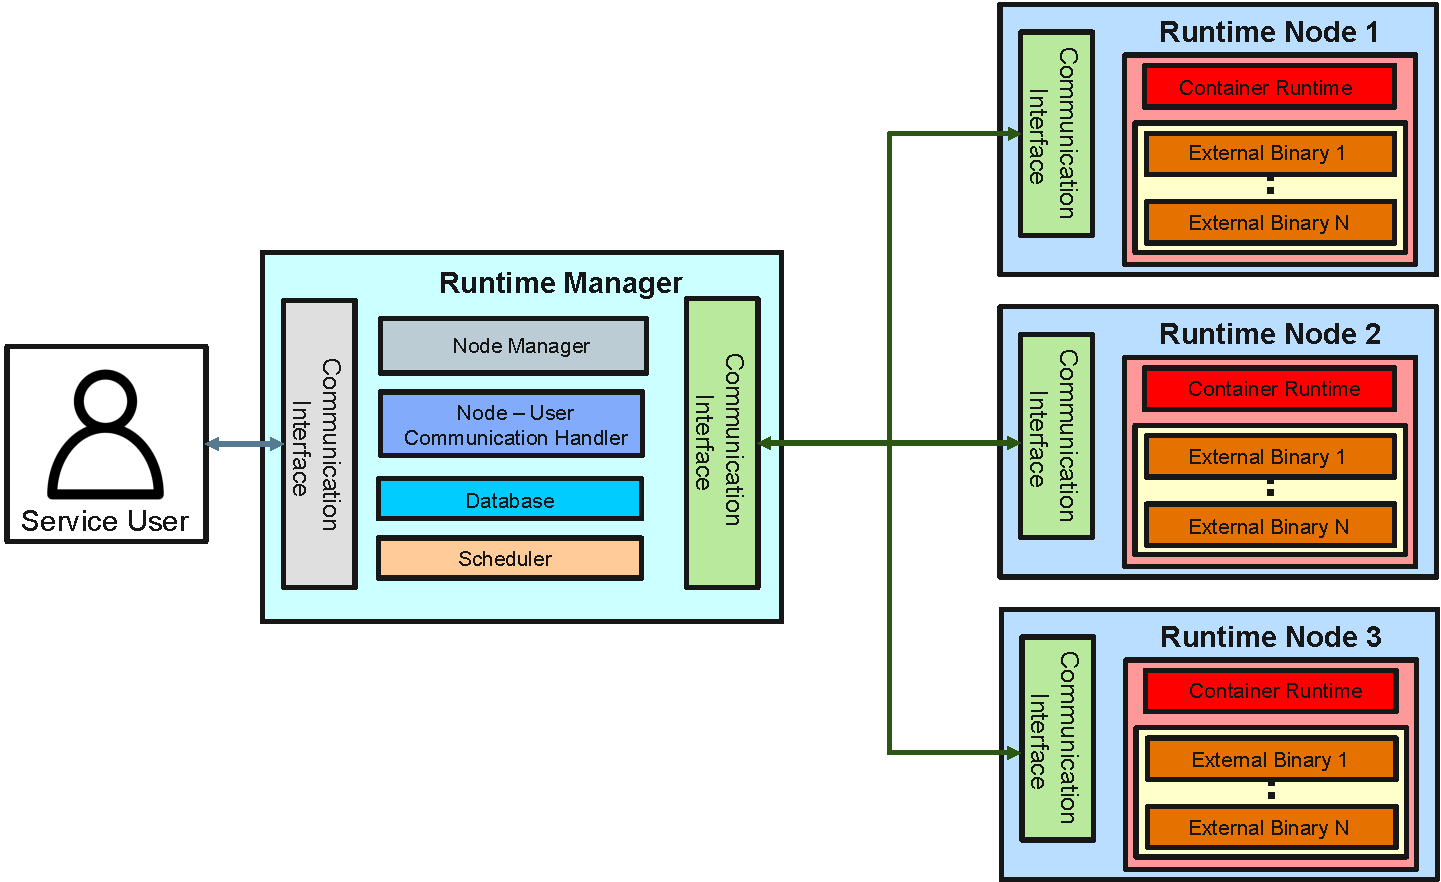
\includegraphics[width=\textwidth]{./content/graphics/Architecture.pdf}
	\caption{Gesamtarchitektur der Softwareplattform}
	\label{architektur}
\end{figure}

\subsection{Runtime Node}

Diese Komponente wird auf den Fahrzeugsteuergeräten ausgeführt und besteht aus mehreren Softwarekomponenten. Die Gesamtarchitektur der Komponente Runtime Node ist in der \autoref{runtime node} dargestellt. Die Kommunikationsschnittstelle ist als eigenständige Softwarekomponente implementiert, die nicht Teil der Softwarekomponente Runtime Node ist. Diese Struktur ermöglicht einen einfachen Austausch der Kommunikationsschnittstelle und damit einen einfachen Wechsel des Kommunikationsprotokolls. Die Kommunikation zwischen der Kommunikationsschnittstelle und dem Runtime Node erfolgt über eine Interprozesskommunikationsschnittstelle. Diese ist im \autoref{Kommunikation zwischen Softwaremodulen} detailliert beschrieben. 

\begin{figure}[htbp]
	\centering
	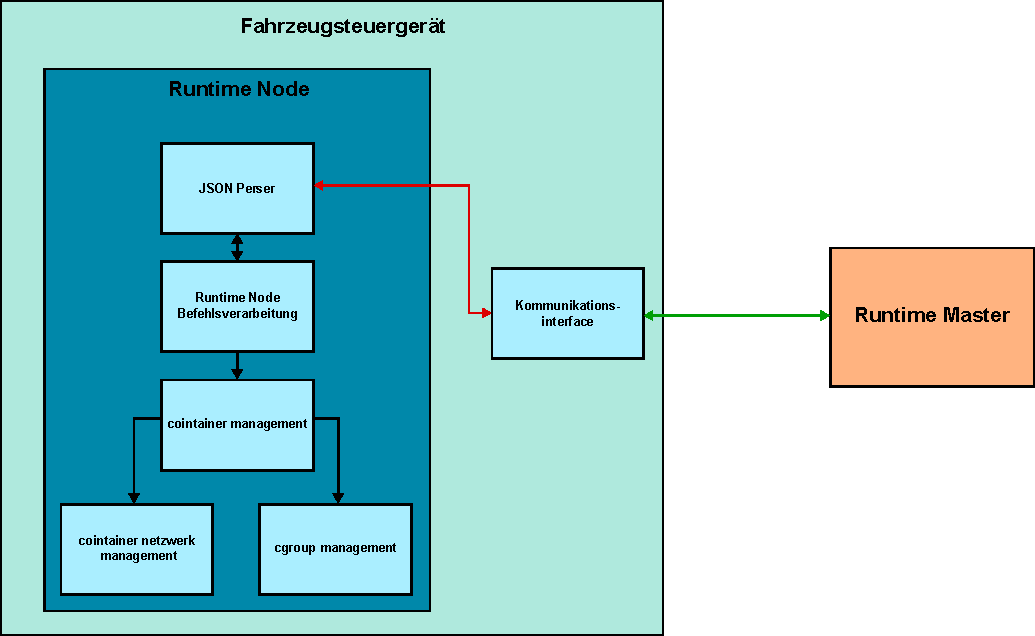
\includegraphics[width=\textwidth]{./content/graphics/Runtime_Node_Arch.pdf}
	\caption{Runtime Node Struktur}
	\label{runtime node}
\end{figure}

\subsubsection{Runtime Node Befehlsverarbeitung}

Diese Komponente interpretiert die Befehle der Kommunikationsschnittstelle und erzeugt Statusrückmeldungen. Abhängig vom empfangenen Befehl ruft sie die entsprechenden Container Management Funktionen auf. Hier werden auch die für den Runtime Master relevanten Informationen und Statusrückmeldungen gesammelt und als Nachricht über die Kommunikationsschnittstelle versendet.

\subsubsection{Container Management}

Die elementare Aufgabe der Softwarekomponente Runtime Node ist die Erzeugung und Verwaltung von isolierten Laufzeitumgebungen. Im \autoref{Virtualisierung} wurde festgelegt, dass diese isolierten Laufzeitumgebungen mit der Virtualisierungsmethode der Containerisierung erzeugt werden. Dabei werden betriebssystemspezifische Isolationsmethoden verwendet, die vom Linux-Kernel zur Verfügung gestellt werden. Konkret werden die in \autoref{Software Virtualisierung/Container} vorgestellten Namespaces verwendet. 

Die Komponente Container Management kann diese isolierte Laufzeitumgebung (Container) erstellen, starten, stoppen und löschen. Diese Aktionen können durch entsprechende Befehle ausgelöst werden, die über die Kommunikationsschnittstelle empfangen werden. Wird ein Befehl zur Erstellung eines Containers empfangen, wird die Erstellung der Laufzeitumgebung angestoßen. Die Isolierung erfolgt zunächst auf Dateisystemebene. Für jeden Container wird ein eigener Ordner angelegt, der als Wurzelverzeichnis konfiguriert wird. Prozesse, die im jeweiligen Container ausgeführt werden, haben nur Zugriff auf die Daten in diesem Verzeichnis. Entsprechend werden auch die benötigten Softwarebibliotheken und Frameworks in diesem Ordner abgelegt, damit sie den Anwendungen innerhalb des Containers zur Verfügung stehen. Dies kann entweder durch die Erstellung eines vorkonfigurierten Ordners erfolgen, der lokal auf dem Steuergerät zur Verfügung steht, oder durch die Übertragung von extern auf die gleiche Weise wie externe Applikationen. Zusätzlich wird der Container in einer lokalen Datenbank registriert, in der Name, Status und vorhandene ausführbare Anwendungen eingetragen werden. Diese Informationen werden an den Runtime Master übertragen, so dass das System einen Überblick über die Container hat.

Wird ein Container gestartet, erzeugt Runtime Node einen neuen Prozess. Dieser Prozess ist der Initialisierungsprozess des Containers, alle Isolierungsmaßnahmen für diesen Prozess gelten auch für die weiteren Prozesse, die von diesem Prozess gestartet werden. Der Container als isolierte Laufzeitumgebung entsteht dadurch, dass dieser Initialisierungsprozess die notwendige Isolierung vom Betriebssystem erhält und die weiteren Prozesse startet, die im Container ausgeführt werden sollen. Die Isolierung erfolgt durch die Verwendung von Namespaces, die vom Linux-Kernel zur Verfügung gestellt werden. Die folgenden Namespace-Isolationsmethoden sind standardmäßig vorgesehen:

\begin{itemize}
    \item NEWNS: Isoliert die Mount-Namespaces oder Mounts. Dateipfade, die dem Prozess durch mount hinzugefügt werden, haben keinen Einfluss auf das zugrunde liegende Betriebssystem.
    \item NEWPID: Isoliert die \gls{PID} des Prozesses, so dass der aktuelle Prozess die \gls{PID} 1 erhält. Dadurch wird dieser Prozess zum Initialisierungsprozess in dieser Umgebung. Andere Prozesse, die nicht vom Initialisierungsprozess in diesem Container gestartet wurden, sind innerhalb des Containers nicht sichtbar.
    \item NEWUTS: Isoliert die Prozess-IDs vom Rest des Systems. Dadurch können Prozesse in der isolierten Umgebung beliebig umbenannt werden, ohne dass es zu Konflikten mit gleichnamigen Prozessen im restlichen System kommt.
    \item NEWNET: Isoliert den Prozess vom Netzwerk-Stack des Host-Systems. Netzwerkadapter, IP-Adressen, Routing-Tabellen, Firewall-Einstellungen und Sockets werden nicht mit dem Host-System geteilt. Prozesse im Container können keine Netzwerkressourcen des Hostsystems verwenden oder dessen Einstellungen einsehen.
\end{itemize}

Um den Zugriff des Containers auf die explizit vorgesehenen Dateipfade zu beschränken, ist eine zusätzliche Routine Pivot Root erforderlich. Pivot Root legt das Wurzelverzeichnis für den Prozess fest, so dass dieser nicht auf hierarchisch übergeordnete Ordnerstrukturen im Dateisystem zugreifen kann. Wird der für den Container spezifisch angelegte Ordner als Root-Verzeichnis definiert, so können die Prozesse auch nur auf Inhalte in diesem Ordner zugreifen. In Kombination mit dem isolierten Mount-Namespace werden die Zugriffsrechte der Prozesse auf die explizit gesetzten Dateipfade beschränkt.

Um die Rechenressourcen des Containers einzuschränken und die durch den Initialisierungsprozess gestarteten Prozesse zu identifizieren, wird die in \autoref{Software Virtualisierung/Container} vorgestellte Linux Feature Control Group (cgroup) verwendet. Die Container-Management-Komponente des Laufzeitknotens legt für den Initialisierungsprozess eine neue cgroup an. Prozesse, die vom Initialisierungsprozess gestartet werden, sind automatisch Teil der cgroup des Initialisierungsprozesses. Dieser Mechanismus ermöglicht es einerseits, die zur Verfügung stehenden Rechenressourcen des Containers bei Bedarf einzuschränken, und andererseits, die im Container laufenden Prozesse eindeutig zu identifizieren. Im Falle eines externen Stoppbefehls für den Container können so alle Prozesse des Containers beendet werden.

Prozesse, die im Container laufen, sind standardmäßig durch die Verwendung von Namespaces vom Hostsystem Netzwerk isoliert. Sollen Anwendungen im Container auf Netzwerkressourcen des Systems zugreifen, kann dies mit Hilfe von Netzwerkbrücken realisiert werden. Dazu werden zwei virtuelle Netzwerkschnittstellen erzeugt, eine Schnittstelle im Namespace des Containers und die andere im Hostsystem. Die Netzwerkbrücke verbindet die beiden Netzwerkschnittstellen und ermöglicht die Netzwerkkommunikation der Container Prozesse im Hostsystem. 

\subsection{Runtime Master}

Die Runtime Master Komponente verwaltet die Runtime Nodes im Gesamtsystem. Das aktuelle Konzept sieht eine laufende Instanz von Runtime Master im System vor. Im gegensatz zu den Runtime Nodes wird diese Komponente nicht auf einem Fahrzeug ausgeführt, sondern auf einem Server. Runtime Master erkennt und verwaltet alle Runtime Node Instanzen im gleichen Netzwerk. Wie Runtime Node besteht auch Runtime Master aus mehreren Softwarekomponenten. Eine Übersicht ist in \autoref{runtime master} dargestellt. Die Kommunikationsschnittstelle ist bei Runtime Node ebenfalls eine separate Softwarekomponente, die nicht teil von Runtime Node ist. 

\begin{figure}[htbp]
	\centering
	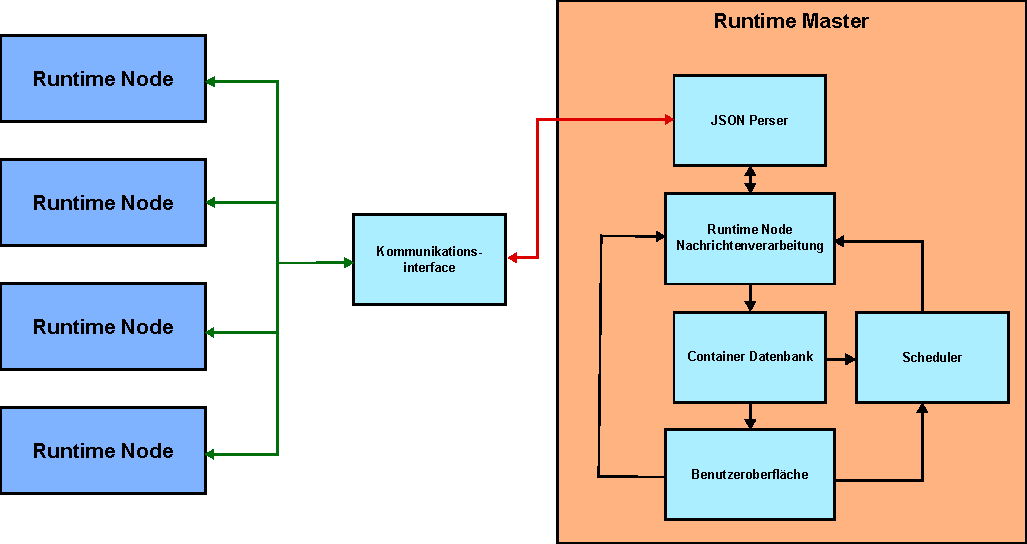
\includegraphics[width=\textwidth]{./content/graphics/Runtime_Master_Arch.pdf}
	\caption{Runtime Master Struktur}
	\label{runtime master}
\end{figure}

\subsubsection{Runtime Master Nachrichtenverwaltung}

Diese Komponente generiert die Befehle, die über die Kommunikationsschnittstelle an die Runtime Nodes übertragen werden und empfängt die Statusmeldungen der Runtime Nodes. Die Befehle können sowohl über eine Benutzeroberfläche manuell oder über eine Scheduler Algorithmus ausgelöst werden. Die Statusmeldungen der Runtime Nodes werden an die Datenbank oder, falls es sich um eine Fehlermeldung handelt, an die Benutzerschnittstelle oder den Scheduler gesendet. 

\subsubsection{Scheduler}

Der Scheduler verteilt die Anwendungen auf die Runtime Nodes. Dabei soll die Verteilung so erfolgen, dass die Last sinnvoll auf die Knoten verteilt wird und eine möglichst effiziente Ausführung erreicht wird. 

\subsubsection{Container Datenbank}

 Informationen über die im Netzwerk vorhandene Runtime Nodes werden in einer Datenbank gespeichert. Dieser kann dafür verwendet werden, dass der Scheduler Informationen über die Runtime Nodes sammeln kann, die für die Verteilung der Applikationen relevant sind. 

\subsection{Kommunikation}

Innerhalb des Systems findet Kommunikation sowohl zwischen den Fahrzeugen als auch zwischen den einzelnen Softwarekomponenten statt. Diese unterschiedlichen Kommunikationsarten stellen unterschiedliche Anforderungen an die verwendete Kommunikationsschnittstelle. Diese werden im folgenden Abschnitt dargestellt.

\subsubsection{Kommunikation zwischen Fahrzeugen und Runtime Master}

Die Fahrzeuge bilden ein verteiltes System, das von einer Runtime Master Instanz verwaltet wird. Dies entspricht einer klassischen Client/Server Kommunikationsstruktur. Die Kommunikation zwischen Fahrzeugen (Runtime Nodes) und Runtime Master wird voraussichtlich über eine Internetverbindung realisiert. Denkbar wäre auch ein vom Fahrzeughersteller bereitgestelltes Netzwerk, das ähnlich der Internetverbindung über das Mobilfunknetz zur Verfügung gestellt wird. In dieser Arbeit wird generell davon ausgegangen, dass sich Fahrzeuge und Runtime Master im selben Netzwerk befinden. 

Für die Client/Server Kommunikation existieren bereits verschiedene Konzepte. Die folgenden Methoden werden häufig verwendet:

\begin{itemize}
    \item Request/Response: Client sendet Anfragen an einen Server und wartet auf Antwort
    \item Publish/Subscribe: Publisher versenden Nachrichten zu einem definierten Thema. Subscriber erhalten die Nachrichten zu den Themen, die sie abonniert haben.
    \item Websocket: Duplex Kommunikation über eine \gls{TCP} Verbindung. 
    \item \gls{RPC}: Ermöglicht die Ausführung eines Prozesses auf einem anderen System, als ob es sich um ein lokales System handeln würde.
\end{itemize}

Hauptsächlich finden zwei verschiedene Kommunikationsarten zwischen Runtime Node und Runtime Master statt. Einerseits werden die Anweisungen an die Runtime Nodes über eine \gls{API} Schnittstelle vom Runtime Master übertragen, andererseits müssen die externe Applikationen an die Runtime Nodes übertragen werden. 

Die Kommunikation mit \gls{API} Schnittstellen wird häufig in Form von Request/Response über das \gls{HTTP} Protokoll realisiert. Hierfür stehen zahlreiche Tools und Softwarebibliotheken zur Verfügung. Die Kommunikation kann auch verschlüsselt erfolgen. 

Das \gls{SOA} Architekturmuster gewinnt in der Informationstechnologie zunehmend an Popularität, da es die effiziente Koordination verteilter Ressourcen und die Wiederverwendbarkeit einzelner Komponenten verbessert. Dieses Muster ist auch Gegenstand der Forschung für Fahrzeugarchitekturen, da diese ebenfalls als verteilte Systeme betrachtet werden können, in denen einzelne Teilnehmer für unterschiedliche Funktionalitäten wiederverwendbar gestaltet werden müssen. Es ist davon auszugehen, dass zukünftige Fahrzeugarchitekturen diesem oder einem ähnlichen Ansatz folgen werden. Als Kommunikationsprotokoll eignet sich für \gls{SOA} Architekturen ein Protokoll, das eine lose Kopplung der einzelnen Komponenten erlaubt und die Anzahl der Teilnehmer dynamisch variieren kann. In diesen Konzepten wird häufig das Publish/Subscribe Konzept verwendet. Publisher können jederzeit Informationen zu einem bestimmten Thema (Topic) veröffentlichen. Alle Subscriber, die das Thema abonniert haben, erhalten die Daten. Die Anzahl der Subscriber und Publisher kann sich während des Betriebs dynamisch ändern, Publisher können ihre Daten auch dann publizieren, wenn es von keinem Subscriber abonniert wurde. Im Gegensatz zum Request/Response Verfahren müssen sich Subscriber und Publisher nicht kennen. Dieses Konzept erlaubt somit eine lose Kopplung und einfache Skalierbarkeit der Kommunikationsteilnehmer. Viele Implementierungen von Publish/Subscribe Kommunikationsprotokollen beinhalten \gls{QoS} Regeln in den übertragenen Nachrichten. In verteilten Systemen, wie sie in \gls{SOA} Architekturen vorkommen, haben die Teilnehmer unterschiedliche Anforderungen an die übertragenen Informationen. Um potentielle Probleme bei der Mehrfachnutzung der gleichen Daten zu vermeiden, können mit Hilfe von \gls{QoS} Regeln bestimmte Garantien definiert werden. Teilnehmer, die auf die Daten zugreifen, können anhand dieser Informationen überprüfen, ob die Daten ein für ihre Funktionalitäten geeignetes Verhalten aufweisen. Je nach Implementierung kann die Anzahl der definierbaren \gls{QoS} Regeln variieren. Als Beispiel kann eine der am weitesten verbreiteten Publish/Subscribe Implementierungen namens \gls{MQTT} betrachtet werden. Diese Implementierung stellt eine \gls{QoS} Regel zur Verfügung, die definiert, wie Nachrichten an Teilnehmer übermittelt werden. Die folgenden 3 Stufen können verwendet werden:

\begin{itemize}
    \item \gls{QoS} 0: Nachricht wird höchstens einmal gesendet, Abonnenten, die zum Zeitpunkt des Sendens das Thema der Nachricht nicht abonniert haben, erhalten die Nachricht nicht.
    \item \gls{QoS} 1: Nachricht wird mindestens einmal gesendet, Nachricht wird kontinuierlich wiederholt, bis ein Teilnehmer eine Empfangsbestätigung zurücksendet.
    \item \gls{QoS} 2: Nachricht wird genau einmal übertragen. Nachricht wird zunächst im Broker zwischengespeichert und an alle Teilnehmer gesendet. Erst wenn alle Abonnenten den Empfang bestätigt haben, wird die Nachricht gelöscht und die erfolgreiche Übertragung an den Publisher gesendet. 
\end{itemize}

Bei der Konfiguration von Nachrichten kann der \gls{QoS}-Level festgelegt und damit das Übertragungsverhalten der Nachricht konfiguriert werden. Andere Implementierungen können auch mehrere definierbare \gls{QoS}-Regeln enthalten, um eine noch genauere Abstimmung der Anforderungen zwischen den Kommunikationsteilnehmern zu ermöglichen. Die Publish/Subscribe Implementierung \gls{DDS} bietet 22 Kategorien von konfigurierbaren \gls{QoS} Regeln. Die zusätzlichen Regeln erlauben es, weitere Anforderungen wie maximale Latenz, Lebensdauer oder Zuverlässigkeit der Nachrichten zu definieren. 

Publish/Subscribe-Systeme können entweder von einer zentralen Instanz, einem so genannten Broker oder Message Bus, oder ohne zentrale Instanz verwaltet werden. Wird eine zentrale Verwaltungsinstanz verwendet, verbinden sich alle Teilnehmer mit dieser Instanz. Publisher übermitteln ihre Nachrichten an diese Administration, Subscriber abonnieren Themen bei der Administration. Die Nachrichten werden entsprechend an die Abonnenten weitergeleitet. Die gesamte Kommunikation in dieser Topologie läuft über diese zentrale Instanz, diese verwaltet die Kommunikationsteilnehmer und Nachrichtenfluss.

Bei der dezentralen Umsetzung entfällt die zentrale Verwaltungsinstanz. Die Teilnehmer kommunizieren direkt miteinander, welches zwei Vorteile mit sich bringt. Zum einen erhöht sich die Robustheit des Systems durch den Wegfall der zentralen Administration, zum anderen verringert sich die Latenz und der Bandbreitenbedarf im Netzwerk durch die direkte Kommunikation. Die Komplexität wird jedoch dadurch erhöht, dass die Netzwerkteilnehmer die anderen Teilnehmer selbst entdecken 
müssen und die Publisher selbst dafür verantwortlich sind, ihre Nachrichten an alle Abonnenten zu übermitteln. Die Erkennung der Teilnehmer erfolgt durch periodische Broadcast Nachrichten, die an alle Netzwerkteilnehmer übermittelt werden. Durch diese Discovery Nachrichten werden Publisher darüber informiert, welche Netzwerkteilnehmer ihre Nachrichten Abonnieren. Die Übertragung der Nachrichten an die Abonnenten erfolgt gezielt an die Netzwerkteilnehmer die das entsprechende Thema abonnieren. Ein Nachteil dieser Methode ergibt sich aus den per Broadcast übertragenen Discovery Nachrichten. Broadcast Nachrichten werden im gesamten Netzwerk an alle Netzwerkteilnehmer verteilt. Dies kann in großen Netzwerken zu einem hohen Bandbreitenverbrauch führen. Aus diesem Grund werden Broadcasts im Internet nicht verwendet, da sie aufgrund der großen Anzahl von Geräten sehr ineffizient wären. Die dezentrale Implementierung mit Broadcast Nachrichten zur Erkennung weiterer Teilnehmer ist aus diesem Grund für die Kommunikation über das Internet nicht nutzbar. Um dieses Problem zu umgehen, bieten dezentrale Publish/Subscribe Implementierungen oft auch die Möglichkeit, Discovery Nachrichten an vorkonfigurierte Adressen zu senden. In diesem Fall müssen die Adressen allen potentiellen Teilnehmern zur Konfigurationszeit bekannt sein, so dass das Netzwerk nicht so flexibel erweiterbar ist.

In der prototypischen Implementierung wird davon ausgegangen, dass sich die serviceorientierte Architektur im Automobil durchsetzen wird, insbesondere bei autonomen Fahrzeugen. Auch der Zusammenschluss vieler Fahrzeuge zu einer verteilten Recheneinheit kann als serviceorientierte Architektur verstanden werden. Aus diesem Grund wurde für die Kommunikation zwischen den Fahrzeugen (Runtime Nodes) und dem Runtime Master die Kommunikationsmethode Publish/Subscribe gewählt. Konkret wurde die \gls{DDS} Implementierung gewählt, da diese durch den Wegfall der zentralen Administration eine einfachere Konfiguration ermöglicht. Diese prototypische Implementierung wird zunächst nur im lokalen Netzwerk betrieben, so dass die Verwendung von Broadcast Messages zur Erkennung von Netzwerkteilnehmern kein Problem darstellt. Die grundlegende Konfiguration der Nachrichten ist für alle Publish/Subscribe Implementierungen gleich, Nachrichten haben ein definiertes Thema und ein Datenfeld, wo Variablennamen und Datentypen in der Nachricht definiert werden können. Dies kann mit geringem Aufwand auf andere Publish/Subscribe Implementierungen übertragen werden, ohne dass die Nachrichten angepasst werden müssen. Bei der Verwendung von \gls{QoS} Regeln ist jedoch zu beachten, dass diese implementierungsspezifisch und daher oft nicht auf andere Implementierungen übertragbar sind. Erfolgt die Kommunikation über das Internet, kann eine Publish/Subscribe Implementierung mit zentraler Verwaltung wie \gls{MQTT} verwendet werden, ohne dass die Struktur der Nachrichten angepasst werden muss. 

Die Publish/Subscribe Methode eignet sich aufgrund der Nachrichtenstruktur gut für die Übertragung von Statusmeldungen oder Befehlen. Ein spezifischer Befehl kann ein eigenes Topic haben, Parameter können im Datenfeld der Nachricht übertragen werden. Für kleine Netzwerke kann die Konfiguration vereinfacht werden, indem für jeden Befehl ein Topic erstellt wird, das von allen Runtime Nodes abonniert wird. Bei diesem Ansatz erhalten alle Runtime Nodes im Netzwerk ein Befehl vom Runtime Master. Die Information, an welchen Runtime Node das Befehl konkret gerichtet ist, kann im Datenfeld als Parameter übermittelt werden. Runtime Nodes, für die das Befehl nicht bestimmt war, erhalten die Nachricht und ignorieren das Befehl nach Prüfung des Datenfeldes. Dieser Ansatz ist ähnlich wie die Nutzung von Broadcast Nachrichten mit dem Unterschied, dass nur alle Runtime Nodes das Netzwerkpaket mit der Nachricht bekommen und nicht alle Netzwerkteilnehmer. Dies ermöglicht, wie bei der Erkennung neuer Teilnehmer, eine einfache Erweiterung des Netzwerkes um neue Teilnehmer ohne zusätzlichen Konfigurationsaufwand. Nachteilig ist jedoch wie beim Broadcast die zunehmende Ineffizienz bei steigender Teilnehmerzahl. Für größere Netzwerke kann die Konfiguration so angepasst werden, dass jeder Runtime Node eigene Topics für seine Befehle verwendet. Dies kann erreicht werden, indem die Topics der Runtime Nodes durch eine zusätzliche eindeutige Kennung ersetzt werden. Diese Kennung kann je nach Implementierung vom Kommunikationsprotokoll bereitgestellt werden, \gls{DDS} vergibt an jeden neuen Teilnehmer eine \gls{GUID}, die nur einmal im Netzwerk existiert. Diese GUID kann an die Topics angehängt werden, so dass sie für jeden Runtime Node eindeutig sind. Nicht jede Publish/Subscribe-Implementierung bietet einen eindeutigen Identifikator, wie ihn \gls{DDS} mit \gls{GUID} implementiert. Im Allgemeinen hat jede Ethernet-Netzwerkschnittstelle eine \gls{MAC} Adresse, Mobilfunk-Netzwerkschnittstellen eine \gls{IMEI}, die für das Gerät eindeutig ist und auch als Teil des Topics verwendet werden kann. Somit können auch unabhängig von der Publish/Subscribe Implementierung individuelle Topics für die Runtime Nodes erstellt werden. 

Für die prototypische Implementierung wurde auf individuelle Topics für die Runtime Nodes verzichtet, da diese Implementierung nicht in großen Netzwerken eingesetzt wird. Eine spätere Modifikation ist jedoch ohne Anpassung der Architektur oder der Grundkonzepte möglich. 

Die zweite Art der Kommunikation ist die Übertragung von Anwendungen. Dieses Konzept sieht vor, dass diese im Binärformat als kompilierte ausführbare Datei vorliegen. Die Übertragung von kompilierten ausführbaren Dateien ist auch ein häufiges Szenario in der \gls{IT}. Für diesen Fall gibt es daher bereits verschiedene Übertragungsprotokolle. Das Kommunikationsprotokoll \gls{HTTP}/\gls{HTTPS}, das hauptsächlich für die Bereitstellung von Web-Inhalten verwendet wird, unterstützt die Übertragung von Dateien. Speziell für den Dateitransfer wurde das Protokoll \gls{FTP} entwickelt. Aufgrund fehlender Sicherheitsmechanismen wird dieses Protokoll nicht mehr bevorzugt eingesetzt. Für die reine Datenübertragung wird als sichere Alternative das auf dem \gls{SSH} Protokoll basierende \gls{SFTP} bevorzugt.

Die Übertragung von Binärdaten ist ebenfalls über Publish/Subscribe Kommunikation realisierbar. Wie für die Übertragung von Befehlen kann auch für die Übertragung von Binärdaten ein Topic definiert werden. Dies kann ebenfalls je nach Systemgröße ein Topic für alle Teilnehmer sein, oder ein individuelles Topic pro Teilnehmer um die Übertragungseffizienz im Netzwerk zu steigern. 

Zusammenfassend kann gesagt werden, dass die Publish/Subscribe-Kommunikationsmethode sowohl die Übertragung von Instruktionen und Statusinformationen als auch die Übertragung von Binärdaten effizient umsetzen kann. Gleichzeitig bietet dieses Konzept eine einfache Erweiterbarkeit für das Netzwerk.

\subsubsection{Kommunikation zwischen Softwaremodulen}
\label{Kommunikation zwischen Softwaremodulen}

Im Kapitel \autoref{Forschungsansatz} wurde erarbeitet, dass die Software einen modularen Aufbau haben soll. Die Komponenten können auch auf demselben PC ausgeführt werden, so dass eine Kommunikationsmethode verwendet werden muss, die die Kommunikation zwischen Prozessen auf demselben System ermöglicht. Für die Interprozesskommunikation können verschiedene Möglichkeiten genutzt werden. Die folgenden Methoden werden von den meisten Betriebssystemen unterstützt und häufig verwendet:

\begin{itemize}
    \item Datei: Datei: Informationen werden in eine Datei auf dem Datenträger geschrieben. Mehrere Prozesse können auf diese Datei zugreifen und ihren Inhalt lesen und schreiben.
    \item Sockel: Daten werden über Netzwerkinterface ausgetauscht. Die Prozesse können sowohl auf dem gleichen System oder Systemübergreifend über Netzwerk kommunizieren. Synchronisierung muss in den Prozessen implementiert werden.
    \item Message Queue: Prozesse können Nachrichten über Message Queues austauschen. Die Übertragung erfolgt asynchron, Sender und Empfänger müssen nicht gleichzeitig aktiv sein. Nicht empfangene Nachrichten werden zwischengespeichert. 
    \item Pipe: Pipes können entweder die unidirektionale Standardeingabe und -ausgabe oder ein ähnliches Verhalten wie eine geteilte Datei implementieren. Für eine bidirektionale Datenaustausch können zwei Pipes verwendet werden. Nicht ausgelesene Daten werden auch bei dieser Methode zwischengespeichert. 
    \item Shared Memory: Mehrere Prozesse können auf denselben Speicherbereich zugreifen, der für den Datenaustausch zwischen den Prozessen genutzt werden kann.
\end{itemize}

Die verschiedenen Kommunikationsmethoden bieten unterschiedliche Vorteile, so dass je nach Anwendungsfall abgewogen werden muss, welche Methode am besten geeignet ist. Bei der Softwareplattform ergeben sich folgende Anforderungen hinsichtlich der Kommunikation zwischen Softwaremodulen:

\begin{itemize}
    \item Übertragung von Befehlen und Statusmeldungen, bidirektionale Kommunikation der Komponenten erforderlich
    \item Softwarekomponenten sind im Betriebszustand alle aktiv, keine asynchrone Kommunikation notwendig
    \item Keine hohen Latenzanforderungen. Das aktuelle Konzept sieht keine Anwendungen vor, die sehr niedrige Latenzen erfordern.
    \item Vorteilhaft ist eine möglichst hohe Flexibilität bezüglich der Ausführungsumgebung und des Ausführungsortes.
\end{itemize}

Aufgrund dieser Anforderungen wurde die Socket-Methode als Kommunikationsschnittstelle gewählt. Diese Methode implementiert eine asynchrone und bidirektionale Kommunikation. Sie kann sowohl auf einem lokalen System als auch systemübergreifend im Netzwerk eingesetzt werden. Somit können Softwarekomponenten, die über Sockets kommunizieren, bei Bedarf auf andere Systeme ausgelagert werden. 

\subsubsection{Kommunikationsformat zwischen Softwarekomponenten}

Die unter \autoref{Kommunikation zwischen Softwaremodulen} aufgeführten Kommunikationsmethoden implementieren nur die Funktionalität, dass Rohdaten ausgetauscht werden können. Das Format, in dem die Daten übertragen werden, muss vom Softwareentwickler implementiert werden. Innerhalb der Software liegen die Daten in den unterstützten Datentypen vor, in vielen Fällen gebündelt als Struct oder Class. Grundsätzlich können Daten auch in ihrem nativen Format in binärer Form zwischen Softwarekomponenten übertragen werden. Dies ist die effizienteste Methode, da keine zusätzlichen Konvertierungsschritte für die Übertragung notwendig sind und keine zusätzliche Datengröße benötigt wird. Nachteilig ist, dass die Daten auf Bit genau von beiden Teilkomponenten gleich interpretiert werden müssen. Dies ist insbesondere dann nicht immer der Fall, wenn die Softwarekomponenten in unterschiedlichen Programmiersprachen entwickelt wurden oder auf unterschiedlichen Systemen laufen. Darüber hinaus erschwert ein solches Konzept die dynamische Erweiterung der übertragenen Daten um zusätzliche Datenfelder bei gleichzeitiger Abwärtskompatibilität zu älteren Softwarekomponenten. Aus diesem Grund werden für die Kommunikation zwischen Softwaremodulen in der Regel keine Rohdaten ausgetauscht, sondern andere Nachrichtenformate verwendet. Diese Formate werden \gls{IDL} oder Schnittstellenbeschreibungssprachen genannt. Folgende Formate finden häufig Anwendung:

\begin{itemize}
    \item \gls{JSON}: Textbasiertes Format, von Menschen unmittelbar lesbar, hierarchische Struktur
    \item \gls{XML}: Textbasiertes Format, von Menschen unmittelbar lesbar, Label-basierte Struktur
    \item Protocol Buffers: Binärformat, kompakt, Nachrichtenstruktur wird durch eine Beschreibungsdatei definiert
    \item MessagePack: Binärformat, ähnliche Struktir wie \gls{JSON} aber nicht von menschen lesbar, kompakt
    \item \gls{YAML}: Textbasiertes Format, von Menschen unmittelbar lesbar, kann komplexe Strukturen darstellen
\end{itemize}

Die aufgeführten Kommunikationsformate bieten je nach Anwendungsfall unterschiedliche Vorteile. Die folgende Tabelle gibt einen Überblick über die Unterschiede zwischen den aufgeführten Methoden:
\begin{table}
    \centering
    \begin{tabular}{|c||c|c|c|c|c|}
        \hline
        \textbf{Eigenschaft} & \textbf{YAML} & \textbf{JSON} & \textbf{Protobuf} & \textbf{MessagePack} & \textbf{XML} \\
        \hline
        \hline
        Kompaktheit & Gering & Mittel & Hoch & Hoch & Gering \\
        \hline
        unmittelbar lesbar & Ja & Ja & Nein & Nein & Ja \\
        \hline
        Parsing Geschwindigkeit & Langsam & Mittel & Schnell & Schnell & Langsam \\
        \hline
    \end{tabular}
    \caption{Vergleich der häufig verwendeten \gls{IDL} Methoden}
\end{table}

In der prototypischen Implementierung werden zwischen Softwarekomponenten hauptsächlich Befehle und Statusmeldungen ausgetauscht. Es ergeben sich hierdurch die Folgenden Anforderungen:

\begin{itemize}
    \item Einfaches Debugging ohne zusätzliche Tools Vorteilhaft
    \item Größe der übertragenen Daten gering
    \item Häufigkeit der Kommunikation gering
\end{itemize}

Aufgrund der Anforderungen wurde die Schnittstellenbeschreibungssprache \gls{JSON} gewählt. Die zusätzliche Kompaktheit der Binärformate ist bei der gegebenen Häufigkeit der Kommunikation und der Menge der übertragenen Daten nicht so entscheidend. Die unmittelbare Lesbarkeit der Daten erleichtert die Fehlersuche im System.

Eine Ausnahme stellt die Übertragung von Binärdaten dar. Diese werden oft nicht in einer Nachricht übertragen, sondern auf mehrere Nachrichten verteilt. Während der Übertragung werden also Nachrichten mit großen Datenfeldern in kurzen Zeitabständen übertragen. Für diesen Anwendungsfall ist die schnelle Parsing Geschwindigkeit und Kompaktheit ausschlaggebend. Die direkte Lesbarkeit spielt bei dieser Methode keine Rolle, da binäre Daten für Menschen nicht direkt lesbar sind. Geeignete Methoden für diesen Fall sind sowohl Protobuf als auch MessagePack. Beide Methoden zeichnen sich durch eine hohe Parsing-Geschwindigkeit und eine hohe Kompaktheit aus.

In der prototypischen Implementierung werden derzeit auch die Binärdaten über \gls{JSON} übertragen, um die Kommunikation einheitlich zu halten. Bei einer Weiterentwicklung ist hier jedoch ein Wechsel auf eine andere \gls{IDL} sinnvoll, um die Übertragungsgeschwindigkeit zu erhöhen.

\section{Scheduling}

Das Scheduling hat die Aufgabe, die externen Applikationen so im System zu verteilen, dass eine effiziente Auslastung der Fahrzeuge (Runtime Nodes) erreicht wird. Für diese Verteilung benötigt der Scheduler sowohl Informationen über die Anforderungen der auszuführenden Applikationen als auch über die Eigenschaften der Runtime Nodes in den Fahrzeugen. Um eine effiziente Auslastung für externe Applikationen zu ermöglichen, wurden folgende Anforderungen an den Scheduler identifiziert:

\begin{itemize}
    \item Applikation muss Kompatibel mit der Architektur der Zielhardware sein. Wenn verschiedene Hardwarearchitekturen im Gesamtsystem vorhanden sind, muss die entsprechende Kompatibilität mit der externen Applikation gewährleistet werden. 
    \item Wenn die Anwendung bestimmte Ressourcenanforderungen hat, wie z.B. Speicherbedarf, müssen die Runtime Nodes diese Anforderungen erfüllen.
    \item Die Ressourcenverteilung soll so effizient wie möglich erfolgen, Runtime Nodes müssen dem Runtime Master entsprechend relevante Informationen über ihre aktuell verfügbaren Rechenressourcen mitteilen.o
    \item Die Verbindungsqualität im Netzwerk ist entscheidend für die Übertragung von Anwendungen und Ergebnissen. Netzwerkeigenschaften wie Bandbreite und Latenz der einzelnen Runtime Nodes sind daher für das Scheduling relevant.
    \item Wahrscheinlichkeit von Zustandsänderungen. Parkende Fahrzeuge benötigen sehr geringe Mengen an Rechenressourcen, so dass sie den Großteil ihrer Ressourcen externen Anwendungen zur Verfügung stellen können. Fährt das Fahrzeug los, ändert sich der Zustand so, dass das Fahrzeug nur noch geringe oder gar keine Ressourcen mehr zur Verfügung stellen kann. Für ein effizientes Scheduling ist es sinnvoll, die Wahrscheinlichkeit des Zustandswechsels abzuschätzen.
    \item Identifizierung und Authentifizierung der Runtime-Knoten. Unberechtigter Zugriff muss verhindert werden und die Runtime Nodes müssen identifizierbar sein.
\end{itemize}

Ausgehend von diesen Anforderungen wurden die folgenden relevanten Informationen ermittelt, die die Runtime Nodes übertragen:

\begin{itemize}
    \item Leistung: 
    \begin{itemize}
        \item CPU Auslastung
        \item Verfügbare Arbeitsspeichermenge
        \item Verfügbare Laufwerkspeichermenge
    \end{itemize} 
    \item Netzwerk:
    \begin{itemize}
        \item Netzwerktyp
        \item Latenz
        \item Position
    \end{itemize}
    \item Characteristic:
    \begin{itemize}
        \item Betriebssystem
        \item CPU Typ und Architektur
        \item Runtime Version
    \end{itemize}
    \item Authentifizierung
    \begin{itemize}
        \item Token
    \end{itemize}
    \item Gesundheitsstatus
    \item Eigenschaften
    \item Zusätzliche Angaben
    \item Vorhandene Container:
    \begin{itemize}
        \item Containername
        \item Containerstatus
        \item Externe Applikationen im Container
    \end{itemize}
\end{itemize}

Mit diesen Informationen können die oben genannten Anforderungen erfüllt werden. Die Authentifizierung ermöglicht eine eindeutige Identifizierung der Knoten. CPU-Typ, Architektur und aktuelle Auslastung ermöglichen die Bestimmung der verfügbaren Rechenleistung im Fahrzeug sowie der Kompatibilität der externen Anwendung mit der Hardware. Der Gesundheitsstatus zeigt an, ob ein Runtime Node ordnungsgemäß funktioniert. Die zusätzliche Angaben und Eigenschaften können weitere Eigenschaften definieren, die für die Verteilung der externen Anwendungen relevant sein können. Die Information über die Netzwerklatenz kann für die Verbindungsqualität verwendet werden. Die Übertragung des Standortes kann z.B. mit Hilfe von Reinforced Learning für die Schätzung von Zustandsänderungen genutzt werden. Dazu können für jedes Fahrzeug statistische Standortdaten erfasst werden, um ein typisches Nutzungsprofil für das Fahrzeug zu ermitteln. Aus dem Nutzungsprofil kann abgeschätzt werden, wann und wie lange das Fahrzeug voraussichtlich stehen wird. 

\subsection{Scheduling Algorithmen}
\label{Scheduling Algorithmen}

Das Scheduling Problem kann im Prinzip als eine erweiterte Form des Knapsack Problems betrachtet werden. Das Knapsackproblem ist ein Modell für Optimierungsprobleme in der Kombinatorik. Es behandelt das Problem, einen Rucksack mit begrenztem Platz mit Gegenständen von unterschiedlicher Größe und Wert zu füllen. Ziel ist es, die Kombination von Gegenständen zu finden, die in den Rucksack passt und den höchsten Gesamtwert aufweist. Dieses Problem weist eine hohe Ähnlichkeit mit Problemen bei der Ressourcenverteilung auf. In diesem Fall müssen Anwendungen, die eine bestimmte Menge an Ressourcen benötigen, auf Systeme mit begrenzt verfügbaren Ressourcen optimal verteilt werden. Das komplette Knapsackproblem geht davon aus, dass jeder Gegenstand beliebig oft vorhanden ist und in beliebiger Menge in den Rucksack gepackt werden kann. Die meisten reale Knapsackprobleme sind sogenannte 0/1 Knapsackprobleme. Das bedeutet, dass ein Objekt genau einmal in der Lösungsmenge enthalten sein kann, es kann nicht in kleinere Teilmengen aufgeteilt werden.Mathematisch lässt sich das Problem durch folgende Formel ausdrücken, für $ i $ Objekte mit jeweils dem Kapazitätsbedarf $ w_i $, der Anzahl in der Lösungsmenge $ x_i $ und der verfügbaren Gesamtkapazität $ W $:

\begin{equation}
    \sum_{i=0}^n w_i x_i  \leq W, x_i \in {0,1} 
    \label{Eq:Knapsack}
\end{equation}

Auch die Verteilung von Anwendungen in einem verteilten Computersystem kann als 0/1 Knapsackproblem aufgefasst werden, da die einzelnen Anwendungen in der Regel nicht aufgeteilt werden können. Zur Lösung von Knapsackproblemen existieren verschiedene Algorithmen. Grundsätzlich kann zwischen Algorithmen unterschieden werden, die eine exakte Optimallösung als Ergebnis garantieren und solchen, die nur eine lokale Optimallösung garantieren. 

\subsubsection{Exakte Algorithmen}

Es existieren verschiedene Methoden, um die exakte optimale Lösung zu finden. Nachfolgend sind einige Beispiele für Algorithmen aufgeführt, die dies ermöglichen. 

Die dynamische Programmierung ist eine weit verbreitete Methode zur Bestimmung der optimalen Lösung des Knapsackproblems. Bei dieser Methode wird eine Tabelle aller Möglichkeiten für Gewicht/Ressourcenverbrauch und Anzahl der Objekte erstellt. In dieser Tabelle werden alle zulässigen Kombinationen berechnet und die Kombination mit dem höchsten Wert ermittelt. Nachfolgend ist die Logik der dynamischen Programmierung als Pseudocode dargestellt. Im dargestellten Fall werden Objekte mit unterschiedlichen Gewichten und Werten betrachtet, wobei die Kombination der Objekte gesucht wird, deren Gesamtgewicht die maximale Kapazität nicht überschreitet und deren Gesamtwert maximal ist:

\begin{algorithmic}
    \State  \textbf{Eingang:} Werte[], gewichte[], Kapazitaet
    \State  \textbf{Ausgang:} Maximaler Gesamtwert
    
    \State  $n \leftarrow$ length(Werte)
    \State  Initialisiere $dp$ ein 2D Array der Größe $(n+1) \times (Kapazitaet+1)$ gefüllt mit 0
    
    \For{$i \leftarrow 1$ to $n$}
        \For{$w \leftarrow 0$ to $Kapazitaet$}
            \If{$Gewichte[i-1] \leq w$}
                \State $dp[i][w] \leftarrow \max(dp[i-1][w], Werte[i-1] + dp[i-1][w - Gewichte[i-1]])$
            \Else
                \State  $dp[i][w] \leftarrow dp[i-1][w]$
            \EndIf
        \EndFor
    \EndFor
    
    \State  \textbf{return} $dp[n][Kapazitaet]$
\end{algorithmic}

In diesem Code wird zuerst die 2D Tabelle der Größe Anzahl Objekte + 1 und Kapazität + 1 erstellt. Die Tabelle ist um einen Index größer als die Anzahl der Objekte und die mögliche Kapazität. Der Grund dafür ist, dass die nachfolgende Logik auf frühere Werte in der Tabelle zurückgreift. Um einen Fehler beim ersten Durchlauf zu vermeiden, beginnt die Schleife bei Index 1, aber Index 0 ist in der Tabelle vorhanden und mit 0 gefüllt. Die Logik besteht aus zwei Schleifen, die erste Schleife iteriert über alle Objekte mit Index $i$, beginnend bei Index 1, um keine Zugriffsverletzung wie oben beschrieben zu erzeugen. Die zweite Schleife iteriert für jeden Objektindex über alle möglichen Gesamtkapazitäten $ w $. 

Bei jeder Iteration wird zunächst geprüft, ob das aktuell ausgewählte Objekt am Index $ i $ in das aktuell ausgewählte Maximalgewicht $ w $ passt. Ist dies der Fall, wird geprüft, ob ein höherer Gesamtwert erreicht werden kann, wenn das aktuelle Objekt zur Lösung hinzugefügt wird. Dazu wird der Wert des neuen Objekts genommen und berechnet, wie viel Kapazität übrig bleibt, wenn das Objekt in die Lösung aufgenommen wird. Anschließend wird für die berechnete Restkapazität der höchste Gesamtwert aus der Tabelle genommen. Zuletzt wird verglichen, ob durch das Hinzufügen des neuen Objekts ein höherer Gesamtwert erreicht wird als vorher. Das Maximum wird als Ergebnis in die Tabelle eingetragen. Überschreitet das Gewicht des neuen Objekts das aktuell zulässige Gesamtgewicht $ w $, wird direkt der vorherige Tabellenwert genommen, da keine Verbesserung mit diesem Objekt möglich ist.

Der Vorteil dieser Methode gegenüber der einfachen \enquote{Brute Force}. Methode, bei der alle möglichen Kombinationen berechnet werden, dass durch die Erstellung der Tabelle bereits berechnete Werte als Zwischenwerte für neue Berechnungen verwendet werden können. Dadurch können redundante Rechenoperationen vermieden werden. Bei $ n $ Objekten und einer Maximalen Kapazität von $ W $ ergeben sich die Berechnungskomplexitäten wie folgt: 

\begin{align}
    & O(2^n) (exponentiell) \\
    & O(nW) (polynomisch)
\end{align}

Aus diesem Zusammenhang ist erkennbar, dass insbesondere bei große Anzahl an Objekten $ n $, erheblich Rechenaufwand durch dynamische Programmierung eingespart werden kann. 

Eine weitere weit verbreitete Alternative zur Berechnung der exakten Lösung ist der Meet-in-the-Middle-Algorithmus. In diesem Algorithmus wird die Gesamtmenge der Objekte in zwei Hälften geteilt. Für diese zwei Hälften werden alle möglichen Kombinationen errechnet, anschließend die Ergebnisse sortiert und zusammengeführt. Der folgende Pseudocode zeigt, wie Meet-in-the-Middle implementiert werden kann:

\begin{algorithmic}
    \State \textbf{Eingang:} Werte[], Gewichte[], Kapazitaet
    \State \textbf{Ausgang:} Maximaler Gesamtwert

    \State $n \leftarrow$ length(Werte)
    \State $Items \leftarrow$ Liste von $(Gewicht, Wert)$ Paaren
    \State Teile $Items$ in $Links$ und $Rechts$

    \State $LinksMengen \leftarrow$ \textsc{GeneriereMengen}($Links$)
    \State $RechtsMengen \leftarrow$ \textsc{GeneriereMengen}($Rechts$)

    \State Sortiere $RechtsMengen$ nach Gewicht
    \State $RechtsMengen \leftarrow$ \textsc{EntferneDominiertePaare}($RechtsMengen$)

    \State $MaxWert \leftarrow 0$
    \ForAll{($wL$, $vL$) in $LinksMengen$}
        \If{$wL \leq Kapazitaet$}
            \State $Rest \leftarrow Kapazitaet - wL$
            \State $vR \leftarrow$ \textsc{BinaereSucheMaxWert}($RechtsMengen$, $Rest$)
            \State $MaxWert \leftarrow \max(MaxWert, vL + vR)$
        \EndIf
    \EndFor

    \State \textbf{return} $MaxWert$

\end{algorithmic}

Zuerst wird eine Liste erstellt, in der die Objektwerte und Gewichte als Paar gespeichert werden. Diese Liste wird in zwei Hälften geteilt. Die Funktion \enquote{GeneriereMengen} berechnet alle möglichen Kombinationen für jede Hälfte und speichert sie in den Variablen \enquote{LinksMengen} und \enquote{RechtsMengen}. Die \enquote{RechtsMengen} werden nach Gewicht sortiert. Die Funktion \enquote{EntferneDominiertePaare} entfernt aus den \enquote{RechtsMengen} alle Kombinationen, bei denen mindestens eine andere Kombination bei geringerem Gewicht einen höheren Gesamtwert erzielt. Diese können ausgeschlossen werden, da sie nicht Teil der optimalen Lösung sein können. Anschließend wird für jedes \enquote{LinksMengen}-Paar geprüft, ob es die Gesamtkapazität überschreitet und wenn nicht, wird die noch verfügbare Restkapazität berechnet. Die Funktion \enquote{BinaereSucheMaxWert} sucht den höchstmöglichen Wert in \enquote{RechtsMengen} für diese verfügbare Restkapazität. Abschließend wird der Gesamtwert der Kombination berechnet und geprüft, ob ein besseres Ergebnis als der bisherige Maximalwert erzielt werden konnte. Ist dies der Fall, wird das aktuelle Ergebnis als Maximalwert gespeichert, andernfalls wird der vorherige Maximalwert beibehalten. Beispielhafte Implementierungen für die verwendeten Hilfsfunktionen sind im folgenden Abschnitt aufgeführt:

\begin{algorithmic}
    \State \vspace{0.5em}
    
    \Function{GeneriereMengen}{$Items$}
    \State $Mengen \leftarrow$ leere Liste
    \State $n \leftarrow$ Länge von $Items$
    \For{$Maske \leftarrow 0$ bis $2^n - 1$}
        \State $Wert \leftarrow 0$, $Gewicht \leftarrow 0$
        \For{$i \leftarrow 0$ bis $n - 1$}
            \If{Bit $i$ in $Maske$ gesetzt}
                \State $Gewicht \leftarrow Gewicht + Items[i].Gewicht$
                \State $Wert \leftarrow Wert + Items[i].Wert$
            \EndIf
        \EndFor
        \State Füge $(Gewicht, Wert)$ zu $Mengen$ hinzu
    \EndFor
    \State \Return $Mengen$
    \EndFunction

\end{algorithmic}

Die Funktion \enquote{GeneriereMengen} berechnet alle möglichen Kombinationen von Objekten. Dazu wird eine Maske in einer Schleife verwendet, die von 0 bis zur Anzahl der Objekte - 1 inkrementiert wird. Für jede Schleife werden der Gesamtwert und das Gesamtgewicht aller Objekte addiert, deren Indexposition $ i $ in der Maske eine 1 ist. Diese Methode stellt sicher, dass alle möglichen Kombinationen berechnet werden. Die Ergebnisse werden in einer Liste \enquote{Mengen} gespeichert und zurückgegeben.

\begin{algorithmic}
    \State \vspace{0.5em}

    \Function{EntferneDominiertePaare}{$Mengen$}
    \State Sortiere $Mengen$ nach aufsteigendem Gewicht
    \State $Gefiltert \leftarrow$ leere Liste
    \State $MaxWert \leftarrow -\infty$
    
    \ForAll{$(w, v)$ in $Mengen$}
        \If{$v > MaxWert$}
            \State Füge $(w, v)$ zu $Gefiltert$ hinzu
            \State $MaxWert \leftarrow v$
        \EndIf
    \EndFor

    \State \Return $Gefiltert$
    \EndFunction

\end{algorithmic}

Die Funktion \enquote{EntfernenDominiertePaare} entfernt alle Kombinationen, deren Gesamtgewicht höher ist als das von mindestens einer anderen Kombination. Zuerst werden alle Objekte nach Gewicht von leicht nach schwer sortiert. In der anschließenden For-Schleife wird für alle sortierten Kombinationen in der Variablen \enquote{Mengen} geprüft, ob sie einen höheren Wert als den bisherigen Maximalwert haben. Durch die Betrachtung der Objekte mit aufsteigendem Gewicht können wir Kombinationen ausschließen, die einen niedrigeren Wert als den bisherigen Maximalwert haben, da es eine Kombination mit gleichem oder geringerem Gewicht existiert, die einen höheren Gesamtwert hat.

\begin{algorithmic}
    \State \vspace{0.5em}
    
    \Function{BinaereSucheMaxWert}{$Mengen$, $MaxGewicht$}
    \State $Links \leftarrow 0$
    \State $Rechts \leftarrow$ Länge($Mengen$) $- 1$
    \State $BesterWert \leftarrow 0$

    \While{$Links \leq Rechts$}
        \State $Mitte \leftarrow \lfloor(Links + Rechts) / 2\rfloor$
        \State $(w, v) \leftarrow Mengen[Mitte]$
        \If{$w \leq MaxGewicht$}
            \State $BesterWert \leftarrow v$
            \State $Links \leftarrow Mitte + 1$
        \Else
            \State $Rechts \leftarrow Mitte - 1$
        \EndIf
    \EndWhile

    \State \Return $BesterWert$
    \EndFunction
\end{algorithmic}

\enquote{BinaereSucheMaxWert} sucht in der Variablen \enquote{Mengen} den Eintrag mit dem höchsten Wert, dessen Gewicht kleiner oder gleich dem in der Variablen \enquote{MaxGewicht} angegebenen Wert ist. Diese Funktion benötigt eine Eingabemenge, die bereits nach Gewicht aufsteigend sortiert und von dominierten Paaren befreit ist. Die binäre Suche nähert sich dem optimalen Ergebnis an, indem sie den Mittelwert aus einem linken und einem rechten Index bildet und diesen Mittelwert als Objektindex verwendet. Zuerst wird geprüft, ob das ausgewählte Objekt schwerer als das maximal erlaubte Gewicht ist. Ist es schwerer als erlaubt, wird der rechte Index auf die Position Mitte - 1 gesetzt. Die Objekte sind aufsteigend nach Gewicht sortiert, so dass wir sofort alle Objekte rechts vom aktuell betrachteten Index ausschließen können, wenn das Objekt am betrachteten Index bereits zu schwer ist. Ist das betrachtete Objekt nicht zu schwer, wird es als aktuell beste Lösung gespeichert und der linke Index auf Links + 1 gesetzt. Da wir die dominierten Paare aus der Menge entfernt haben, enthält sie für jede vorkommende Gesamtgewicht bereits die Kombination mit dem höchsten Wert. Auf diese Weise können wir Objekte, die leichter als das betrachtete Objekt sind, sofort aus der Lösungsmenge ausschließen, da sie nur einen niedrigeren Wert haben können. Diese Logik wird in einer Schleife ausgeführt, bis die Bedingung Linksindex = Rechtsindex erfüllt ist. Durch diese Bedingung wissen wir, dass alle Objekte rechts vom betrachteten Objekt zu schwer und alle Objekte links vom betrachteten Objekt zu leicht sind und daher nicht den höchsten Wert für das zulässige Gesamtgewicht haben.

Beide Algorithmen berechnen die exakte optimale Lösung des Problems. Welcher der beiden Algorithmen effizienter ist, hängt von der Problemstellung ab. In den vorherigen Abschnitten wurden bereits die Berechnungskomplexitäten angegeben:


    Dynamsiche Programmierung: \\
\begin{align}
    & O(n \cdot W) (pseudo-polynomiell)
    \label{EQ:DP}
\end{align}
    Meet-in-the-Middle: \\
\begin{align}
    & O(2^{(n/2)} \cdot log(2^{(n/2)})) (exponentiell-halbiert)
    \label{EQ:MitM}
\end{align}

Auffällig ist, dass die Komplexität bei Meet-in-the-Middle nur von der Anzahl der Objekte $ n $ abhängt, während bei der dynamischen Programmierung auch die Gesamtkapazität $ W $ in die Komplexität eingeht. Ist die Anzahl der Objekte $ n $ groß, aber die Gesamtkapazität $ W $ klein, so kann die dynamische Programmierung das Endergebnis mit geringerem Rechenaufwand berechnen. Ist $ n $ klein und $ W $ groß, ist Meet-in-the-Middle effizienter.

\subsubsection{Approximationsalgorithmen}

In größeren Systemen sind oft sowohl $ n $ als auch $ W $ groß, so dass exakte Algorithmen wegen des zu hohen Rechenaufwandes nicht effizient eingesetzt werden können. In diesen Fällen wird zugunsten des Rechenaufwandes und der Rechenzeit auf eine exakte Optimallösung verzichtet. Für die Approximation stehen ebenfalls verschiedene Algorithmen zur Verfügung:

Die Greedy Approximierung wurde für das komplette Knapsack Problem entworfen. Im \autoref{Scheduling Algorithmen} wurde der wesentliche Unterschied zum 0/1 Knapsack erklärt, beim vollständigen Knapsack können einzelne Objekte beliebig oft zur Lösungsmenge hinzugefügt werden. Greedy sortiert die Menge der Objekte nach Wert pro Gewicht $ v_1 / w_1 \geq ... \geq v_n / w_n $. Nach der Sortierung nimmt der Algorithmus das Objekt mit dem besten Verhältnis von Wert zu Gewicht und fügt es so oft zur Lösungsmenge hinzu, bis kein Platz mehr für ein weiteres Exemplar vorhanden ist. Grundsätzlich kann Greedy auch für 0/1 Knapsack Probleme angewendet werden, in diesem Fall werden die reihe nach die Objekte mit dem besten Wert pro Gewicht Verhältnis genommen, bis die Maximalkapazität erreicht ist. Greedy Algorithmus für einen 0/1 Knapsack kann z. B. mit folgender Logik implementiert werden:

\begin{algorithmic}
    \Function{GreedyKnapsack}{$Werte$, $Gewichte$, $Kapazitaet$}
    \State $n \leftarrow$ Länge von $Werte$
    \State Erstelle Liste $Items$ mit Tupeln $(Werte[i], Gewichte[i], i)$
    \State Sortiere $Items$ absteigend nach $\frac{Werte}{Gewichte}$
    \State $Gesamtwert \leftarrow 0$
    \State $VerbleibendeKapazitaet \leftarrow Kapazitaet$

    \For{$(Wert, Gewicht, i)$ in $Items$}
        \If{$Gewicht \leq VerbleibendeKapazitaet$}
            \State $Gesamtwert \leftarrow Gesamtwert + Wert$
            \State $VerbleibendeKapazitaet \leftarrow VerbleibendeKapazitaet - Gewicht$
        \EndIf
    \EndFor

    \State \Return $Gesamtwert$
    \EndFunction
\end{algorithmic}

Dieser Code fügt die eingegebenen Werte und Gewichte in einer Liste zusammen und sortiert sie absteigend nach dem Wert/Gewicht Verhältnis. In der Schleife werden die Objekte der Reihe nach der Lösungsmenge hinzugefügt, beginnend mit dem Objekt mit dem besten Wert/Gewicht Verhältnis, bis die maximale Kapazität erreicht ist. Der so ermittelte Gesamtwert wird zurückgegeben. Die Berechnungskomplexität bei Greedy beträgt inklusive Sortierung:

\begin{align}
    & O(n \cdot log(n)) (logarithmisch-linear)
\end{align}

Die Berechnungskomplexität ist im Vergleich zu den Algorithmen die die exakte optimale Lösung liefern (\autoref{EQ:DP}, \autoref{EQ:MitM}) deutlich geringer mit einer logarithmisch-linear ansteigendem Komplexität über die Anzahl der Objekte $ n $. 

Als Approximationsalgorithmus kann auch die dynamische Programmierung verwendet werden. Aus \autoref{EQ:DP} ist bereits bekannt, dass der Rechenaufwand sowohl von der Anzahl der Objekte $ n $ als auch von der maximalen Kapazität $ W $ abhängt. Die  Problemstellung kann allerdings bei dynamische Programmierung auch umformuliert werden. Es kann auch bei gegebenem Maximalwert das Minimalgewicht gesucht werden. In diesem Fall ändert sich die Berechnungskomplexität mit Maximalwert $ V $:

\begin{align}
    & O(n \cdot W)  \rightarrow O(n \cdot V) 
\end{align}

Die Komplexität des Problems kann vereinfacht werden, indem sowohl der Maximalwert als auch die Einzelwerte der Objekte herunterskaliert und gerundet werden.  Die Komplexität der Berechnung kann durch die Einführung eines Fehlerfaktors $ \varepsilon $ reduziert werden. Dieser Faktor bestimmt den maximalen Fehler, der durch die Skalierung auftreten kann, z.B. $ \varepsilon = 0,1 $ führt zu einem maximalen Fehler von $ 10 \% $. Aus dem Fehlerfaktor und dem maximal auftretenden Einzelwert $ V_max $ in den Objekten kann der Skalierungsfaktor $ K $ nach folgender Formel berechnet werden:

\begin{align}
    & K = \frac{\varepsilon \cdot V_{max}}{n}
\end{align}

Mit Hilfe des Skalierungsfaktors $ K $ werden alle Einzelwerte der Objekte skaliert und abgerundet. 

\begin{align}
    & v_i^{\prime} = \lfloor \frac{v_i}{K} \rfloor
\end{align}

Diese Skalierung reduziert die Komplexitiät des Problems auf Kosten der Genauigkeit des Endergebnisses. Den Zusammenhang zwischen Fehlerfaktor und Komplexität zeigt der folgende Formel:

\begin{align}
    & O(\frac{n^2}{\varepsilon})
\end{align}

Aus den obigen Formeln ist ersichtlich, warum das Problem von der ursprünglichen \enquote{Ermittlung des Maximalwertes bei gegebener Maximalkapazität} in \enquote{Ermittlung der Minimalkapazität bei gegebener Gesamtkapazität} umformuliert wurde. Die Skalierung führt zu einem Fehler im berechneten Ergebnis, der tatsächliche Wert nach Auswahl der Kombination kann um den Fehlerfaktor $ \varepsilon $ von der Approximation abweichen. Bei einer Skalierung der Kapazitäten kann es daher vorkommen, dass die berechnete optimale Lösung aufgrund des Skalierungsfehlers die zulässige Maximalkapazität überschreitet. Die umformulierte Tabelle kann dennoch verwendet werden, um den Maximalwert für eine gegebene Kapazität zu bestimmen, indem der höchste Wert, der unter der Maximalkapazität liegt, als Lösung verwendet wird.

